\documentclass[a4paper]{IEEEtran}

\usepackage[fleqn]{amsmath}
\usepackage[hidelinks]{hyperref}
\usepackage{pdflscape}
\usepackage{footnote}

\usepackage{graphicx}
\graphicspath{ {images/} }

\title{CloudOCR: Cloud Computing Large Lab Assignment}
\author{
	\IEEEauthorblockN{Tiago Mota \\}
	\IEEEauthorblockA{Email: neozflux@gmail.com \\}
	\and
	\IEEEauthorblockN{Eddy Bertoluzzo \\}
	\IEEEauthorblockA{Email: eddy.bertoluzzo@gmail.com \\}
	\and
	\IEEEauthorblockN{David Hoepelman\\}
	\IEEEauthorblockA{Email: dhoepelman@gmail.com\\}
	\and
	\IEEEauthorblockN{Course instructors: Alexandru Iosup, Dick Epema\\}
	\IEEEauthorblockA{Email: A.Iosup@tudelft.nl, D.H.J.Epema@tudelft.nl\\}
}
\makesavenoteenv{tabular} 

\begin{document}

\maketitle

\begin{abstract}
In this report we introduce CloudOCR, a cloud-based system for automatic OCR-conversion of image files.
The system is fully automatic, highly customisable and can dynamically scale its resources based on the available workload. CloudOCR bases its resource allocation on Amazon EC2 spot instances in order to keep the costs as low as possible.

We test the scalability, resource allocation and cost effectiveness on different Amazon EC2 instance types of our solution and show that it correctly solves the give use case being cheaper and faster that the correspondent desktop solution.
\end{abstract}

\section{Introduction}


\subsection*{Problem}

WantCloud BV is a library that wants to keep up with the developing technologies of the 21th century. They digitized their existing book collection and started digitally renting them.

Since this first step was a success, they now want to OCR their digital collection, adding features such as searching through, highlighting, or tagging the texts, in order to offer a better service to their customers.

WantCloud BV does not want to build the infrastructure themselves but would rather lease it from a Cloud Provider. Their main concern is keeping costs as low as possible .

The conversion of their existing (large) selection of books is under little time constraint, but they do want to be able to prioritise new books and OCR them very quickly.

\subsection*{Proposed solution}
Using Amazon Web Services as the cloud infrastructure provider, we developed CloudOCR, a cloud-based system for the automatic OCR-conversion of text images.

CloudOCR scales according to the number of available jobs, load-balances the workload evenly across the rented machines (from now on called workers) and provides fault tolerance in both the master and the workers. 

The system is fully automatic, aside from the submission of jobs to the database and the resolution of faulty jobs.

\subsection*{Outline}
We begin with detailing the application used for the OCR-conversion and its requirements in section \ref{sec:backgroundonapplication}. In section \ref{sec:systemdesign} we present the design and implementation of our solution, while in section \ref{sec:experimentalresults} we introduce and discuss the experiments used to evaluate the system. We conclude the report with section \ref{sec:discussion}  and \ref{sec:conclusion} in which we discuss and draw conclusions from the evaluation of our system.

\section{Background on Application}
\label{sec:backgroundonapplication}
CloudOCR is based on a existing technology called Tesseract OCR \cite{tesseractocr}, that provides OCR services for bitmap image files such as ``JPEG'' or ``PNG'' and extracts their content into plain text files. W.l.o.g., our application takes only JPEG image files as input and output a simple text file.

We also make use of the Amazon AWS cloud, specifically EC2 (Virtual Machines), S3 (Storage) and RDS (Relational Database) services.

In order to meet WantCloud BV's requirements, we focused the design of CloudOCR on the following features: 
\begin{LaTeXdescription}
	\item[Automation] Given that WantCloud does not have the human resources to constantly manage the application, CloudOCR should perform normally without any user intervention.
	\item[Elasticity] WantCloud has a large, constantly expanding, library to OCR, therefore the application has be able to scale to large numbers of jobs.
	\item[Performance] Time constraints for the conversion are of little importance, but the costs must be kept as low as possible.
	\item[Reliability] Failures or corrupted jobs should be handled gracefully and should not halt the system.
	\item[Monitoring] Worker numbers and job throughput should be monitored.
	\item[Scheduling] The system should make use of Amazon's spot instance system (wherein one bids for system capacity) to keep costs as low as possible.
\end{LaTeXdescription}

\section{System Design}
\label{sec:systemdesign}

\subsection*{Global overview}

CloudOCR has been implemented following the master-slave pattern. One master server both handles the allocation, scheduling, monitoring (and so on) tasks and controls the slaves (workers) that execute jobs.

One jobs consists of one image file to be processed by Tesseract. Jobs are inserted into an ordered queue which is implemented in a database. The scheduler assigns jobs to workers (at a fixed maximum per worker) and stores the assignments in the database.

Workers pull their jobs from the database and start processing them. The monitor retrieves system information which the scheduler, allocation manager and fault manager can use. The allocation manager monitors the number of available jobs and requests spot instances accordingly. The fault manager monitors the system for faults and reinserts uncompleted jobs of failed machines or removes corrupt jobs.

A high-level diagram can be found in Figure \ref{fig_sysarch}.

\subsection*{System components}

\begin{LaTeXdescription}

\item[Front-End] We use a simple Java program to store new jobs in the queue. As the insertion consists of only a file upload and a SQL query, different front-ends (e.g. on-line) are trivial to implement.

\item[Job Queue]
The job queue holds jobs that still need to be processed and its meta-information such as priority and number of failures. We implemented it using a MySQL database, querying it to get the updated, sorted by priority, job queue.

\item[Job Scheduler]
The scheduler assigns the jobs from the queue to the available workers and includes the logic for \textbf{load-balancing}. A \textbf{greedy on-line load-balancing} algorithm \cite{kleinberg2006} is used to assign these jobs to those workers, until a configurable maximum amount of jobs per worker is reached. The scheduler is executed at regular predefined intervals.

\item[Workers]
Workers exists only to execute jobs and are implemented as Amazon EC2 instances running a common AMI that has the open source OCR engine Tesseract OCR installed. Every time a job is completed, after performing the proper updates in the database, the free worker checks the database, pulls one of its assignments and starts executing it.

\item[System Monitor]
The system monitor keeps track of useful information like worker status or resource usage, in order to provide this information to other system components like the fault and allocation manager.

\item[Fault Manager]
The fault manager waits for fault information about workers or jobs from the monitor and handles them accordingly. Failing VM's are simply shutdown (if they were not already by Amazon) while failed jobs are resubmitted to the job queue. A job that consistently fails is removed from the queue and logged; the maximum number of failures is configurable.

\item[Allocation Manager]
The allocation manager allocates workers according to the number of available jobs. The user can configure the minimum and maximum amount of on-demand workers that the system will allocate (in our experiments, we set it to 1 to keep a minimum throughput while minimizing costs); after the maximum is reached, only spot instances will be requested, if the current price is low enough, according to the provisioning policy.

\item[Provisioning Policy]
The provisioning policy can be easily replaced by implementing a simple interface given as an API to the user; by providing the new implementation class and setting its name in the application configuration, the user can easily customise the behaviour of the system.

\item[CloudOCR.properties]
This file comes with the application and lets the user set all sorts of parameters (e.g. min/max number of on-demand instances, provisioning policy, spot instances max bid and so on) in order to make the system tuneable to the user's needs.

\end{LaTeXdescription}

\subsection*{Resource management}

\begin{LaTeXdescription}
\item[Automation]
The implemented system is completely automated, with the exception of the submission of new jobs and the inspection of consistently failing jobs (which are simply removed from the queue).

\item[Elasticity]
The \textbf{Allocation Manager} handles workers' allocation an deallocation according to a specified, configurable policy, providing automatic resource scaling to the system.

\item[Performance]
The \textbf{Job Scheduler} is responsible for guaranteeing the system load balance by distributing the jobs with an online greedy load-balancing algorithm \cite{kleinberg2006}.

\item[Reliability]
Reliability for the workers and jobs is provided by the \textbf{Fault Manager}, which handles all the failures in workers and its jobs. For the master, there is no reliability provided.

\item[Monitoring]
A dedicated monitoring subsystem keeps track of the workers and aggregates information for other components to use; if necessary, it can also be logged.

\end{LaTeXdescription}

\subsection*{System Policies}

\begin{LaTeXdescription}

\item[Job Allocation]
Users can specify a priority for a job, meaning that jobs will only be chosen by the scheduler when no higher-priority jobs are available. Jobs with the same priority are scheduled according to time they were submitted, which means first in, first out.

\item[Resource Allocation]
A configurable minimum throughput can be configured by allocating on-demand instances. After this number is met, only spot instances will be allocated. The upper limit on allocated resources is set according to the provisioning policy; the current one is set to allocate machines in order for the system to complete all its jobs within a configurable amount of time (one hour in our experiments). 

\end{LaTeXdescription}

\subsection*{Additional System Features}

\begin{LaTeXdescription}
\item[Scheduling]
Our solution focuses on efficient scheduling to minimize the total cost. This is done by the Allocation Manager, using spot instances to keep the total cost as low as possible, while relying on a configurable minimal throughput.
The user can also configure this price/performance trade-off.

\item[Fault management]
Fault management is made easy by the use of the database. A failed Master will be able to reconstruct its state by just querying the database and collecting information through the Amazon APIs while the worker will only need to pull again its assignments from the database.

\item[Smart Resource Deallocation]
The Allocation Manager also performs "deallocation protection", that is, it only shuts down workers for which the user will be charged within a configurable amount of time (e.g. 5 minutes); if it is not able to find any suitable candidates, it will postpone the deallocation, therefore not wasting paid resources and increasing the tradeoff between resource utilisation and instance cost. The deallocation protection also shelters from slowdowns when nearly all jobs are completed, therefore causing many workers to be shut down in a little time.

\end{LaTeXdescription}

\section{Experimental results}
\label{sec:experimentalresults}

\subsection{Experimental Setup}

For our experiments we used Amazon EC2 m1.micro, m1.small and m1.medium instances. Specifications can be found in Table \ref{amazoninstancespec}. All instances were running Ubuntu 13.10 (Linux kernel 3.8.0).

The database was provided by Amazon RDS, which uses the same instance specifications but is slightly more expensive. The OS and RDMS were both controlled by Amazon, we know only that a 64-bit Linux was used by checking the mysql status information. We configured RDS to use MySQL 5.6.13.

To keep tests as comparable as possible we only made use of one file for the jobs, a 450 KB JPEG image with a resolution of 2064x1096, containing 3 scanned book pages (Figure \ref{fig_standardjob}).

We implemented the system as a Java program with seperate entry points for the worker and master. We used sql2o \cite{sql2o} to access the database from Java and SLF4J for the logging \cite{SLF4J}.

\begin{savenotes}
\begin{table}
\caption{Amazon EC2 instance types}
\label{amazoninstancespec}
\centering
\begin{tabular}{| l | l | l | l | l |}
\hline
Type & CPU\footnote{"One EC2 Compute Unit (ECU) provides the equivalent CPU capacity of a 1.0-1.2 GHz 2007 Opteron or 2007 Xeon processor." \cite{amazonecu}} & RAM & I/O speed & On-demand/Spot price\footnote{"The spot price varies due to demand, this is the minimum spot price which we used as the only price we wanted to rent spot instances."} \\ \hline
Micro & \textless 2 ECU & 0.6 GB & Low & 0.02/0.006 \$/hr \\ \hline
Small & 1 ECU & 1.7 GB & Moderate & 0.065/0.016 \$/hr \\ \hline
Medium & 2 ECU & 3.75 GB & Moderate & 0.13/0.032 \$/hr \\ \hline
\end{tabular}
\end{table}
\end{savenotes}

\subsection{Experiments}

\subsubsection{Database performance}

We use a relational database (MySQL) to store our jobs and assignments. As such the database becomes our most probable bottleneck when it comes of scaling. We tested the Amazon RDS database performance with databases containing a different number of jobs and executed the query that is needed to retrieve the jobs for scheduling. To accurately test the bottleneck we retrieved all jobs instead of a number dependent on the number of workers (as the scheduler actually does).

We ran the test concurrently from the same VM to the different instance types to make sure environmental factors were minimized. Our own experiment had previously shown that running the tests concurrently does not have a significant influence on the results. We ran each test 50 times and report the average values.

As it can be seen from the results in Table \ref{dbperfresults} and Figure \ref{fig_dbperfresults}, database overhead only becomes noticeable with at least 100,000 jobs and significant starting from 1,000,000 jobs. As we configured the scheduler to retrieve 10 jobs per active worker this would mean 100,000 workers. We thus conclude that database overhead is not a bottleneck for the scaling of our application.

\begin{figure}
\centering
\includegraphics[width=0.5\textwidth]{"results-database"}
\caption{Average database job retrieval time}
\label{fig_dbperfresults}
\end{figure}

\begin{table}
\caption{Average database job retrieval time}
\label{dbperfresults}
\centering
\begin{tabular}{| l | l | l | l |}
\hline
\# Jobs & Micro & Small & Medium \\ \hline
1000 & 0,004s &	0,003s & 0,007s \\ \hline
10000 & 0,025s & 0,025s & 0,026s \\ \hline
100000 & 0,31s & 0,52s & 0,37s \\ \hline
1000000 & 5,28s & 5,84s & 3,74s \\ \hline
3000000	& 79,46s & 18,87s & 11,61s \\ \hline
\end{tabular}
\end{table}
\ \\
\subsubsection{Instance type selection}

To check which instance type would be the best to use for our workers we ran the same job 50 times on the 3 different instance types. To compare the performance we also ran the test on a relatively standard desktop machine (CPU: Intel Core i7 2670QM, RAM: 16GB, OS: Windows 8.0 x64). The results can be seen in Table \ref{tesperfresults} and Figure \ref{fig_tesperfresults}

Our main findings are that the chosen instance type does not greatly influence the price per job if spot instances are used. For production uses we would have opted for the medium instance type (and tested other instances types to see if they were even cheaper). However to reap the benefits of the free resources provided by Amazon\footnote{Amazon AWS has a "free usage tier" which among other consists of 750 free EC2 micro instance hours and 750 free micro RDS instance hours} we chose to use micro instances in all our development and experiments.
\newline

\begin{figure}
\centering
\includegraphics[width=0.5\textwidth]{"results-tesseract"}
\caption{Average job processing time}
\label{fig_tesperfresults}
\end{figure}

\begin{table}
\caption{Average Tesseract job processing time}
\label{tesperfresults}
\centering
\begin{tabular}{| l | l | l |}
\hline
Instance & Processing time & Cost / job (normal/spot) \\ \hline
Micro & 326s & 0,0018 / 0,00054 \$ \\ \hline
Small & 93s & 0,0017 / 0,00041 \$ \\ \hline
Medium & 45s & 0,0016 / 0,00037 \$ \\ \hline
Desktop & 30s & n.a. \\ \hline
\end{tabular}
\end{table}

\subsubsection{Allocation behavior}

We tested whether CloudOCR had the desired allocation behaviour by simulating a workload. We configured CloudOCR to only use spot instances. We configured the ideal number of workers to be 10\% the number of assigned jobs, which corresponds to completing all jobs in about an hour (see Table \ref{tesperfresults}). We then started the system with 100 jobs available and added 100 jobs more at the 15 minute mark.

Furthermore we decreased the "deallocation protection" from 50 minutes to 10 minutes. The de-allocation protection prevents workers from being deallocated if they have been running fewer than 50 minutes of an hour. This is because Amazon charges for a full hour even if only a portion of an hour is used; this prevents needless wasting of money. We opted for this choice in order to show the deallocation behaviour more clearly. 

As can be seen clearly from the results (Figure \ref{fig_allperfresults}) our application closely follows the configured allocation. It is worth noting the lag appearing when new jobs are submitted to the queue and before the workers become available; this is due to both Amazon requiring some time to fullfill our spot requests and the machines taking a while before booting up. The lag before deallocation is caused the protection mentioned earlier.

\begin{figure}
\centering
\includegraphics[width=0.5\textwidth]{"results-allocation-2"}
\caption{Allocation characteristics with workload 1}
\label{fig_allperfresults}
\end{figure}
 
\section{Discussion}
\label{sec:discussion}

\subsubsection*{Application Scaling}

In the first set of experiments we showed how the database overhead does not bother us with scalability problems. Sadly, due to the great amount of time required for the processing of a production workload and the relative small amount of time we had, we could not explore this aspect in depth. It is worth noting, though, that in all our tests, the CPU usage of the Master hardly ever reached 15\% on a micro Amazon instance type, making it very likely to scale well with the increasing of the number of jobs.

\subsubsection*{Database or Memory}

One of the main concerns in the early development of the application was weather to store the data (e.g. jobs or assignments) in memory or save it on a database. The memory option, on one hand, had the advantages of being faster and causing less overhead in comparison to a RDMS, but, since it does not provide persistence, it would have necessarily caused the need for the implementation of a checkpoint system, in order to provide fault management. A RDMS on the other hand, would have intrinsically both provided data persistence and a major help for the fault management and a simplification of communication mechanisms (sparing us from using RMI or SSH) when sending jobs to the workers. We therefore opted for the RDMS solution in the management of the jobs (i.e. not the workers) and showed that its overhead is not a bottleneck for the scaling of our application.

\subsubsection*{Load Prediction}

As we can see from Figure \ref{fig_allperfresults} the allocation and booting up of a VM takes Amazon a few minutes. This can decrease performance, especially if the load of the application is variable. An improvement for our system would be to incorporate load prediction algorithm, such as the one mentioned in \cite{cloudscale}, in the Allocation Manager, in order to anticipate when the load is going to increase and act consequently. An example would be that of preallocating machines at the startup of the system since we are sure that the system is going to make use of them. Our use-case was too limited to explore this feature properly, so we propose it as future work.

\subsubsection*{Better Load Characteristics}

A major limitation we encountered in the implementation of our system was that of accurately predicting the performance of Tesseract, based on simple file information. We found that both file-size and image resolution have little influence have little influence on the outcomes. Finally, we were forced to load-balance based on file-size of jobs and to provision based on the number of jobs. A better understanding of the performance characteristics of Tesseract w.r.t the input files (by studying its performance on different files) could greatly improve our load-balancing and provisioning.

\subsubsection*{Speed/Cost Trade-Off}

The main speed/cost trade-off of CLoudOCR can be identified in determining how many on-demand instances the system will maximally use. Obviously, this only depends on the user's need, but it is worth to note that a higher number greatly increase cost (when compared to spot instances), but also greatly increase guaranteed throughput. It also decreases the number of failures due to killed VMs (on-demand instances are normally not killed by Amazon).

\subsubsection*{Is a cloud-based solution preferable?}

Based on our cost per job results (see Table \ref{tesperfresults}) we here propose a rough estimate of the costs for  a cloud-based and non-cloud OCR system. The market cost for a typical desktop system is in average \$750 and consumes about 200W of power per hour. We used \$0.25/Kwh as the energy price and the \$0.00037 as the average cost of a job running on a Medium instance. This results in the following calculation for the break-even point of the cost of a desktop and cloud solution:
$$
750\$ + 0.2 \cdot 0.25\$ \cdot \frac{\text{\#Jobs}}{120} = 0.00037\$ \cdot \text{\#Jobs}
$$

The equivalence is reached with a number of jobs well over a million jobs, meaning that the desktop solution would need to run non-stop for over a year in order to compute a dataset that the cloud-based solution would process in a few days. Note that this calculation excludes other costs such as the ones for maintenance and network infrastructure. These results show that a cloud-based solution is very attractive, both in time and cost gains, compared to a desktop system. We do not discuss the option of a private cluster since the costs would raise enormously.
	
\section{Conclusion}
\label{sec:conclusion}
In this report, we designed and presented CloudOCR, an IaaS cloud-based system for OCR-conversion of image files, and evaluated its performance on Amazon Web Services.
Our results show that the designed system performs well in solving the given use-case due to little CPU usage,  smart resource allocation and cost effectiveness. CloudOCR is cheaper and faster than an equivalent desktop solution, with a high level of configurability that makes it the right choice for a large number of different user with different need.

\begin{thebibliography}{9}

\bibitem{kleinberg2006}{
 Algorithm design: Chapter 11, \emph{Kleinberg, Jon and Tardos, Éva}, Pearson/Addison Wesley, Boston (Mass.), ISBN: 0-321-37291-3
 }
 
 \bibitem{cloudscale}{
CloudScale: Elastic Resource Scaling for Multi-Tenant Cloud Systems, \emph{Z. Shen, S. Subbiah, X. Gu, and J. Wilkes},  2nd ACM Symp. on Cloud Computing, 2011.
}
 
\bibitem{amazonecu}{
	Amazon EC2 instance description page:  \url{http://aws.amazon.com/ec2/#instance}
}

\bibitem{tesseractocr} {
	Tesseract OCR: \url{https://code.google.com/p/tesseract-ocr/}
}

\bibitem{sql2o} {
	Sql2o: \url{http://www.sql2o.org/}
}

\bibitem{SLF4J} {
	The Simple Logging Facade for Java (SLF4J) : \url{http://www.slf4j.org/}
}

\end{thebibliography}

\appendix{Time spent}
\newline
\begin{tabular}{| l | l |}
\hline
total-time & 162 hours \\ \hline
think-time & 19 hours \\ \hline
dev-time & 124 hours \\ \hline
analysis-time & 13 hours \\ \hline
wasted-time & 6 hours \\ \hline
\end{tabular}
\\\ 
\\
The wasted time comes from rewriting a portion of the application because we altered the system design.
\newline
\newline
Time spent on experiments:
\newline
\begin{LaTeXdescription}
\item[Database performance] \ \\
\newline
\begin{tabular}{| l | l |}
\hline
total-time & 4 hours \\ \hline
dev-time & 1 hours \\ \hline
setup-time & 3 hours \\ \hline
\end{tabular}
\item[Instance type selection] \ \\
\newline
\begin{tabular}{| l | l |}
\hline
total-time & 4 hours \\ \hline
dev-time & 2 hours \\ \hline
setup-time & 2 hours \\ \hline
\end{tabular}
\newline
\newline
\item[Allocation behavior] \ \\
\newline
\begin{tabular}{| l | l |}
\hline
total-time & 2 hours \\ \hline
dev-time & 1 hours \\ \hline
setup-time & 1 hours \\ \hline
\end{tabular}
\\\ 
\newline
The experiment itself was very simple to set-up, but we had to spend a of time to get the system stable enough to test it for multiple hours.
\end{LaTeXdescription}


\begin{landscape}
\appendix

\begin{figure}[h]
\centering
\includegraphics[width=700pt]{"System Architecture 2"}
\caption{System architecture}
\label{fig_sysarch}
\end{figure}
\end{landscape}
\clearpage

\begin{landscape}
\appendix

\begin{figure}[h]
\centering
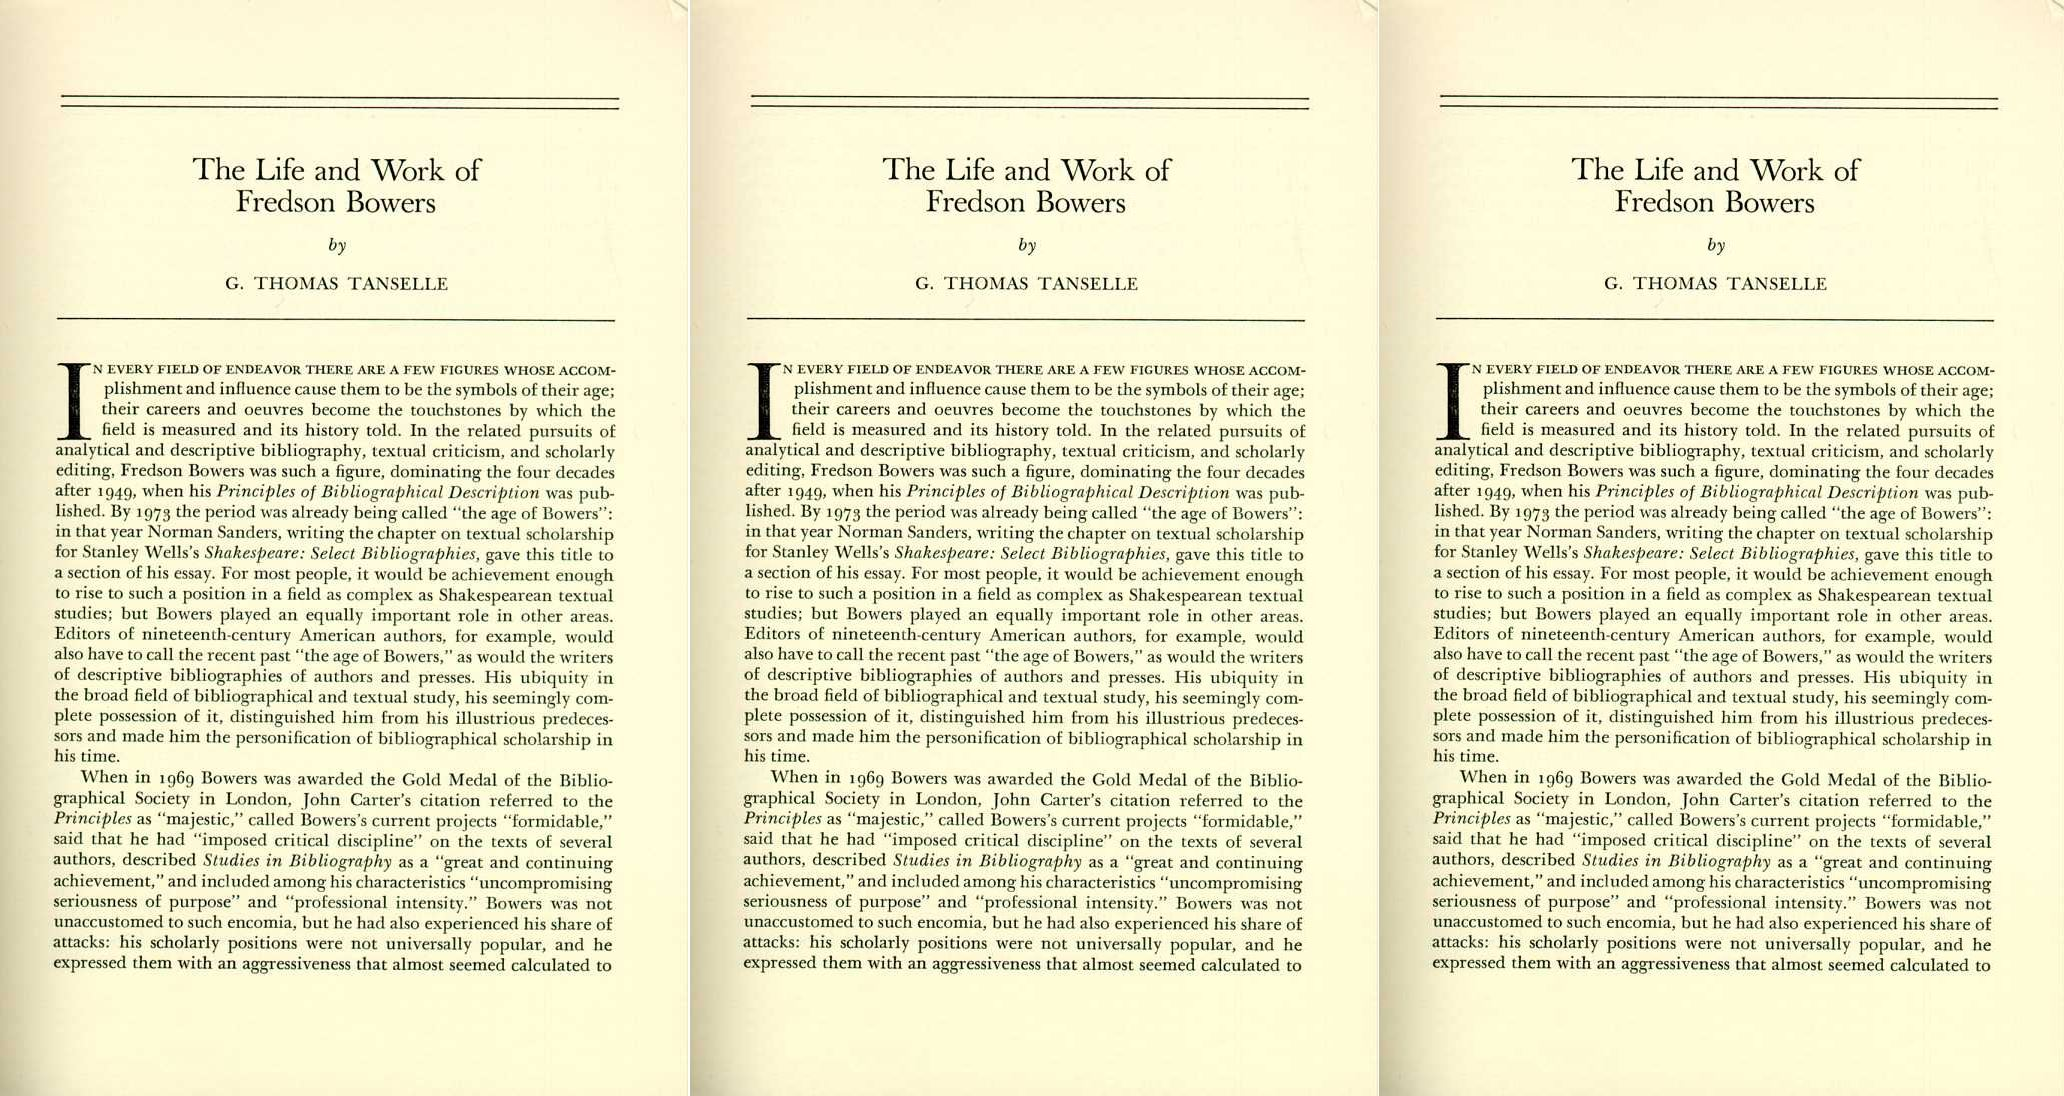
\includegraphics[width=700pt]{standardfile}
\caption{Standard Job image file}
\label{fig_standardjob}
\end{figure}
\end{landscape}
\clearpage

\end{document}